\documentclass[12pt,utf8]{beamer}
\usepackage{graphicx}
\usepackage[ngerman]{babel}
\usepackage[utf8]{inputenc}
\usepackage{amsmath}
\usepackage{amssymb}
\usepackage{listings}
\usepackage{hyperref}
\usepackage{color}

\usepackage[percent]{overpic}

\lstset{literate={ö}{{ \"o}}1
{ü}{{ \"u}}1
{ä}{{ \"a}}1
{ß}{{ \ss}}1
}

\lstset{
language=XML,
basicstyle=\scriptsize,
breaklines=true
}

%Copyright 2008 by Adrian Böhmichen
%
% This file is free software: you can redistribute it and/or modify
% it under the terms of the GNU General Public License as published by
% the Free Software Foundation, either version 3 of the License, or
% (at your option) any later version.
%
% This file is distributed in the hope that it will be useful,
% but WITHOUT ANY WARRANTY; without even the implied warranty of
% MERCHANTABILITY or FITNESS FOR A PARTICULAR PURPOSE.  See the
% GNU General Public License for more details.
%
% You should have received a copy of the GNU General Public License
% along with this file.  If not, see <http://www.gnu.org/licenses/>.

%%%%%%%%%%%%%%%%%%%%%%%%%%%%%%%%%%%%%%%%%%%%%%%%%%%%%%%%%%%%%%%%%
%     Ubuntuusers Vorlage für ein LaTeX-Beamer Theme            %
%                                                               %
% Für das Korrekte funktionieren benötigt man einen header.png  %
% und ein logo.png Datei!                                       %
% Zusätzlich muss man folgende Pakete benutzten:                %
%   \usepackage{graphicx}                                       %
%   \usepackage[percent]{overpic}                               %
%                                                               %
% Danach muss nur noch am Anfang die Datei                      %
% mit \input{} eingebunden werden.                              %
%                                                               %
%%%%%%%%%%%%%%%%%%%%%%%%%%%%%%%%%%%%%%%%%%%%%%%%%%%%%%%%%%%%%%%%%

%weitere Farbe spezifizieren:
%Farben von dem Humantheme
%\definecolor{Orange}{RGB}{240,165,19}
\definecolor{Orange}{RGB}{5,215,242}
%\definecolor{Human-Base}{RGB}{129,102,71}
\definecolor{Human-Base}{RGB}{5,25,242}
%Farben aus dem Inyokatheme
%\definecolor{uuheader1}{RGB}{164,143,101}
\definecolor{uuheader1}{RGB}{5,25,242}
%\definecolor{uuheader2}{RGB}{129,106,59}
\definecolor{uuheader2}{RGB}{5,25,242}


%Theme festlegen für alle Templates die nicht selbstständig definiert werden:
\usepackage{beamerthemedefault}


%Definieren des Innertheme, zuständig für die Symbole bei Listen
\setbeamertemplate{sections/subsections in toc}[square]
\setbeamertemplate{items}[circle]

\setbeamercolor{item}{fg=Human-Base}

%entfernen der Navigationsleiste
\beamertemplatenavigationsymbolsempty

%Logo definieren, man kann die Lage nicht verändern
%\logo{\includegraphics[scale=0.1]{logo.png}}


%Kopf- und Fußzeile definieren
%\setbeamertemplate{headline}
%{%
%\begin{overpic}[width=\paperwidth
% nächste Zeile dient zum anzeigen eines Rasters, für das paltzieren des ToC hilfreich
%,grid,tics=10
%]
%{header.png}%
%  \put(0,11){\insertsectionnavigationhorizontal{\paperwidth}{~}{~}}%
%  \end{overpic}
%}

\setbeamertemplate{footline}[text line]
{%
\begin{minipage}[b]{116mm}
\insertauthor \hfill%
%neue Navigationsleiste
 \insertframenumber ~/ \inserttotalframenumber\\[1ex]
\end{minipage}
}

% Farben festlegen ausserhalb des innertheme

%Allgemeine Angaben und Verbesserung vom default Theme
\setbeamercolor{structure}{fg=uuheader1}
\setbeamercolor{section in toc}{fg=Human-Base}
\setbeamercolor{subsection in toc}{parent=section in toc}
\setbeamercolor{framesubtitle}{fg=uuheader2}


%Farbe und Form der Blöcke definieren
\setbeamertemplate{blocks}[rounded]
%\setbeamercolor{block title}{fg=uuheader1,bg=Orange}
%\setbeamercolor{block title alerted}{use=alerted text,fg=black,bg=alerted text.fg!75!bg}
%\setbeamercolor{block title example}{use=example text,fg=black,bg=example text.fg!75!bg}

%\setbeamercolor{block body}{parent=normal text,use=block title,bg=block title.bg!25!bg}
%\setbeamercolor{block body alerted}{parent=normal text,use=block title alerted,bg=block title alerted.bg!25!bg}
%\setbeamercolor{block body example}{parent=normal text,use=block title example,bg=block title example.bg!25!bg}

%Für den Titleframe
\setbeamertemplate{title page}[default][rounded=true]
\setbeamercolor{title}{fg=uuheader2,bg=Orange}


\begin{document}
\title{Algorithmen und Analyse auf bibliographischen Daten}   
\author{peterr und Lusy} 
\date{\today} 

\begin{frame}
	\titlepage
\end{frame}

\begin{frame}
	\frametitle{Eigenschaften des Datensatzes}
	\begin{itemize}
		\item  enthält ca. $700\,000$ Einträge 
		\item  mit 19 verschiedenen Themengebieten(setSpecs) z.B. cs, math 
		\item  nur der Themenbereich Physik wird in Themengruppen aufgeteilt
		\item  11 Einträge haben keine Metadaten und damit keinen Titel, Autor usw.
	\end{itemize} 
\end{frame}
\begin{frame}[fragile]
	\frametitle{Aufbau der Datensatz}
	\begin{block}{Header}
	\begin{lstlisting}[language=HTML]
		<identifier>oai:arXiv.org:0704.0001</identifier>
		<datestamp>2008-11-26</datestamp>
		<setSpec>physics:hep-ph</setSpec>
	\end{lstlisting}
	\end{block}
	\begin{block}{Metadaten}
		\begin{lstlisting}
		  <dc:title>Titel des Papers</dc:title>
		  <dc:creator>Author 1</dc:creator>
		  <dc:creator>Author 2</dc:creator>
		  <dc:subject>..</dc:subject>
		  <dc:description>Beschreibung</dc:description>
		  <dc:description>Comment</dc:description>
		  <dc:date>2007-04-02</dc:date>
		  <dc:date>2007-07-24</dc:date>
		  <dc:type>text</dc:type>
		  <dc:identifier>http://arxiv.org/abs/0704.0001</dc:identifier>
		  <dc:identifier>Phys.Rev.D76:013009,2007</dc:identifier>
		\end{lstlisting}
	\end{block}
\end{frame}
\begin{frame}
	\frametitle{Parsen der Daten}
	\begin{itemize}
		\item  Parser in Python geschrieben 
		\item  kompletter Datensatz in den Speicher
		%\begin{itemsize}
		%	\item Overhead des XML-Parser vergessen
		%\end{itemsize}
		\item  nur der Themenbereich Physik wird in Themengruppen aufgeteilt
		\item  11 Einträge haben keine Metadaten und damit keinen Titel, Autor usw.
	\end{itemize}
\end{frame}
\begin{frame}
	\frametitle{Verteilung der Themen}
	\begin{center}
		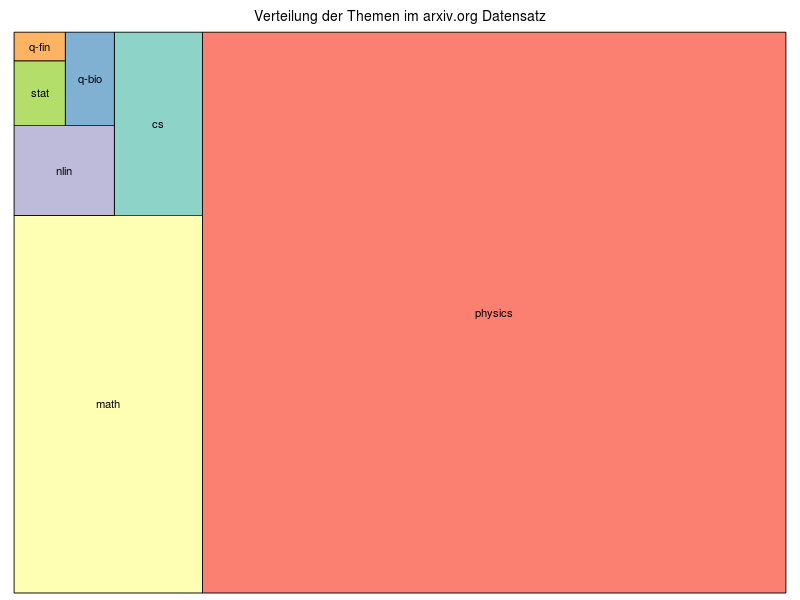
\includegraphics[scale=0.35]{../visual/treeParent.png}
	\end{center}
\end{frame}
\begin{frame}
	\frametitle{Aufschlüsselung von physics}
	\begin{center}
		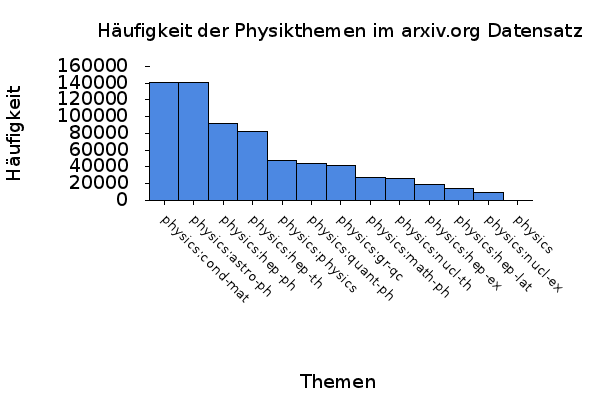
\includegraphics[scale=0.45]{../visual/setSpecFreq.png}
	\end{center}
\end{frame}
\begin{frame}
	\frametitle{Häufigkeit von Themen pro Publikation}
\end{frame}
\begin{frame}
	\frametitle{Assoziationsregeln auf setSpec}
\end{frame}
\begin{frame}
	\frametitle{Probleme}
\end{frame}
\begin{frame}
	\frametitle{Weitere Analysen}
\end{frame}
\end{document}
